\documentclass[ignorenonframetext, compress, 9pt, xcolor=svgnames]{beamer} 
\usepackage{pdfpages}
\usepackage{amsmath}
\usepackage{amsfonts}
\usepackage{amssymb}
\setbeamercolor{frametitle}{fg=DarkBlue}
\setbeamercolor{sectionpage title}{bg=DarkBlue}
%\setbeamercolor{section in head/foot}{bg=DarkBlue}
%\setbeamercolor{author in head/foot}{bg=DarkBlue}
\setbeamercolor{author in head/foot}{fg=DarkBlue}
%\setbeamercolor{title in head/foot}{bg=White}
\setbeamercolor{title in head/foot}{fg=DarkBlue}
%\setbeamercolor{date in head/foot}{fg=Brown}
%\setbeamercolor{alerted text}{fg=DarkBlue}
%\usecolortheme[named=DarkBlue]{structure} 
%\usepackage{bbm}
%\usepackage{bbold}
\usepackage{eurosym}
\usepackage{graphicx}
%\usepackage{epstopdf}
\usepackage{hyperref}
\hypersetup{
  colorlinks   = true, %Colours links instead of ugly boxes
  urlcolor     = blue, %Colour for external hyperlinks
  linkcolor    = blue, %Colour of internal links
  citecolor   = blue %Colour of citations
}
\usepackage{multirow}
\usepackage{xspace}
\usepackage{listings}
\usepackage{natbib}
\usepackage{booktabs}
\usepackage{dcolumn}
%\usepackage[greek,frenchb]{babel}
\usepackage[utf8]{inputenc}
\usepackage[T1]{fontenc}
\usepackage{natbib}
\renewcommand{\cite}{\citet}
\usepackage{longtable}
\setbeamertemplate{caption}[numbered]
\setbeamertemplate{theorem}[ams style]
\setbeamertemplate{theorems}[numbered]
%\usefonttheme{serif}
%\usecolortheme{beaver}
%\usetheme{Hannover}
%\usetheme{CambridgeUS}
%\usetheme{Madrid}
%\usecolortheme{whale}
%\usetheme{Warsaw}
%\usetheme{Luebeck}
\usetheme{Montpellier}
%\usetheme{Berlin}
%\setbeamercolor{titlelike}{parent=structure}
%\setbeamertemplate{headline}[default]
%\setbeamertemplate{footline}[default]
%\setbeamertemplate{footline}[Malmoe]
%\setbeamercovered{transparent}
%\setbeamercovered{invisible}
%\usecolortheme{crane}
%\usecolortheme{dolphin}
%\usepackage{pxfonts}
%\usepackage{isomath}
%\usepackage{mathpazo}
%\usepackage{arev} %     (Arev/Vera Sans)
%\usepackage{eulervm} %_   (Euler Math)
%\usepackage{fixmath} %  (Computer Modern)
%\usepackage{hvmath} %_   (HV-Math/Helvetica)
%\usepackage{tmmath} %_   (TM-Math/Times)
%\usepackage{tgheros}
%\usepackage{cmbright}
%\usepackage{ccfonts} \usepackage[T1]{fontenc}
%\usepackage[garamond]{mathdesign}

%\usepackage{color}
%\usepackage{ulem}

%\usepackage[math]{kurier}
%\usepackage[no-math]{fontspec}
%\setmainfont{Fontin Sans}
%\setsansfont{Fontin Sans}
%\setbeamerfont{frametitle}{size=\LARGE,series=\bfseries}

% suppress navigation bar
\beamertemplatenavigationsymbolsempty
%\usetheme{bunsenMod}
%\setbeamercovered{transparent}
%\setbeamertemplate{items}[circle]
%\usecolortheme[named=CadetBlue]{structure}
%\usecolortheme[RGB={225,64,5}]{structure}
%\definecolor{burntRed}{RGB}{225,64,5}
%\setbeamercolor{alerted text}{fg=burntRed} 
%\usecolortheme[RGB={0,40,110}]{structure}
%\hypersetup{linkcolor=burntRed}
%\hypersetup{urlcolor=burntRed}
%\hypersetup{filecolor=burntRed}
%\hypersetup{citecolor=burntRed}

%\usetheme{bunsenMod}
%\setbeamercovered{transparent}
%\setbeamertemplate{items}[circle]
%\usecolortheme[named=CadetBlue]{structure}
%\usecolortheme[RGB={225,64,5}]{structure}
%\definecolor{burntRed}{RGB}{225,64,5}
%\setbeamercolor{alerted text}{fg=burntRed} 
%\usecolortheme[RGB={0,40,110}]{structure}
%\hypersetup{linkcolor=burntRed}
%\hypersetup{urlcolor=burntRed}
%\hypersetup{filecolor=burntRed}
%\hypersetup{citecolor=burntRed}

%\AtBeginSection[] % Do nothing for \section*
%{ \frame{\sectionpage} }
%\setbeamertemplate{frametitle continuation}{}
\newtheorem{lemme}{Lemme}[section]
\newtheorem{remarque}{Remarque}
\newcommand{\argmax}{\operatornamewithlimits{arg\,max}}
\newcommand{\argmin}{\operatornamewithlimits{arg\,min}}
\def\inprobLOW{\rightarrow_p}
\def\inprobHIGH{\,{\buildrel p \over \rightarrow}\,} 
\def\inprob{\,{\inprobHIGH}\,} 
\def\indist{\,{\buildrel d \over \rightarrow}\,} 
\def\sima{\,{\buildrel a \over \sim}\,} 
\def\F{\mathbb{F}}
\def\R{\mathbb{R}}
\newcommand{\gmatrix}[1]{\begin{pmatrix} {#1}_{11} & \cdots &
    {#1}_{1n} \\ \vdots & \ddots & \vdots \\ {#1}_{m1} & \cdots &
    {#1}_{mn} \end{pmatrix}}
\newcommand{\iprod}[2]{\left\langle {#1} , {#2} \right\rangle}
\newcommand{\norm}[1]{\left\Vert {#1} \right\Vert}
\newcommand{\abs}[1]{\left\vert {#1} \right\vert}
\renewcommand{\det}{\mathrm{det}}
\newcommand{\rank}{\mathrm{rank}}
\newcommand{\spn}{\mathrm{span}}
\newcommand{\row}{\mathrm{Row}}
\newcommand{\col}{\mathrm{Col}}
\renewcommand{\dim}{\mathrm{dim}}
\newcommand{\prefeq}{\succeq}
\newcommand{\pref}{\succ}
\newcommand{\seq}[1]{\{{#1}_n \}_{n=1}^\infty }
\renewcommand{\to}{{\rightarrow}}
\renewcommand{\L}{{\mathcal{L}}}
\newcommand{\Er}{\mathrm{E}}
\renewcommand{\Pr}{\mathrm{P}}
%\newcommand{\Var}{\mathrm{Var}}
\newcommand{\Cov}{\mathrm{Cov}}
\newcommand{\corr}{\mathrm{Corr}}
%\newcommand{\Var}{\mathrm{Var}}
\newcommand{\bias}{\mathrm{Bias}}
\newcommand{\mse}{\mathrm{MSE}}
\providecommand{\Pred}{\mathcal{P}}
\providecommand{\plim}{\operatornamewithlimits{plim}}
\providecommand{\avg}{\frac{1}{n} \underset{i=1}{\overset{n}{\sum}}}
\providecommand{\sumin}{{\sum_{i=1}^n}}
\providecommand{\limp}{\overset{p}{\longrightarrow}}
\providecommand{\limp}{\underset{n \rightarrow \infty}{\overset{p}{\longrightarrow}}}
%\providecommand{\limp}{\underset{n \rightarrow \infty}{\overset{p}{\longrightarrow}}}
\providecommand{\limp}{\overset{p}{\longrightarrow}}
%\providecommand{\limd}{\underset{n \rightarrow \infty}{\overset{d}{\longrightarrow}}}
\providecommand{\limd}{\overset{d}{\longrightarrow}}
\def\independenT#1#2{\mathrel{\setbox0\hbox{$#1#2$}%
    \copy0\kern-\wd0\mkern4mu\box0}} 
\newcommand\indep{\protect\mathpalette{\protect\independenT}{\perp}}


\lstset{language=R}
\lstset{keywordstyle=\color[rgb]{0,0,1},                                        % keywords
        commentstyle=\color[rgb]{0.133,0.545,0.133},    % comments
        stringstyle=\color[rgb]{0.627,0.126,0.941}      % strings
}       
\lstset{
  showstringspaces=false,       % not emphasize spaces in strings 
  columns=fixed,
  numbersep=3mm, numbers=left, numberstyle=\tiny,       % number style
  frame=none,
  framexleftmargin=5mm, xleftmargin=5mm         % tweak margins
}
\makeatletter
%\setbeamertemplate{frametitle continuation}{\gdef\beamer@frametitle{}}
\setbeamertemplate{frametitle continuation}{\frametitle{}}
\makeatother

\newtheorem{theoreme}{Théorème}
\newtheorem{proposition}{Proposition}
\newtheorem{corollaire}{Corollaire}
\newtheorem{exemple}{Exemple}
\newtheorem{assumption}{Assumption}
\renewcommand{\theassumption}{A\arabic{assumption}}
\newtheorem{hypothese}{Hypothèse}
\renewcommand{\thehypothese}{H\arabic{hypothese}}
\newcommand{\Var}{\mathrm{Var}}
\renewcommand{\Er}{\mathbb{E}}
\newcommand{\LP}{\mathcal{LP}}
\providecommand{\Id}{\mathbf{I}}
\providecommand{\Rang}{\mathrm{Rang}}
\providecommand{\Trace}{\mathrm{Trace}}
\renewcommand{\Cov}{\mathrm{Cov}}
\providecommand{\Corr}{\mathrm{Corr}}
\providecommand{\Diag}{\mathrm{Diag}}
\providecommand{\reg}{\mathrm{r}}
\providecommand{\Likelihood}{\mathrm{L}}
\renewcommand{\Pr}{{\mathbb{P}}}
\providecommand{\set}[1]{\left\{#1\right\}}
\providecommand{\uvec}{\mathbf{1}}
\providecommand{\Rang}{\mathrm{Rang}}
\providecommand{\Trace}{\mathrm{Trace}}
\providecommand{\Tr}{\mathrm{Tr}}
\providecommand{\CI}{\mathrm{CI}}
\providecommand{\asyvar}{\mathrm{AsyVar}}
\newcommand{\se}{\mathrm{SE}}
\newcommand{\inputslide}[2]{{
    \usebackgroundtemplate{
      \includegraphics[page={#2},width=\paperwidth,keepaspectratio=true]
      {{#1}}}
    \frame[plain]{}
  }}
\newcommand\pperp{\perp\!\!\!\perp}
\usepackage{bbm}
\providecommand{\Ind}{\mathbf{1}}
\newcommand{\sumjsi}{\underset{i<j}{{\sum}}}
\newcommand{\prodjsi}{\underset{i<j}{{\prod}}}
\newcommand{\sumisj}{\underset{j<i}{{\sum}}}
\newcommand{\prodisj}{\underset{j<i}{{\prod}}}
\newcommand{\sumobs}{\underset{i=1}{\overset{N}{\sum}}}
\newcommand{\prodobs}{\underset{i=1}{\overset{N}{\prod}}}
%\newcommand{\sumobs}{\sum_{i=1}^N}
%\newcommand{\prodobs}{\prod_{i=1}^N}
%\newcommand{\sumjsi}{\sum_{i<j}}
%\newcommand{\prodjsi}{\prod_{i<j}}
%\newcommand{\sumisj}{\sum_{j<i}}
%\newcommand{\prodisj}{\sum_{j<i}}

\usepackage{appendixnumberbeamer}
\setbeamertemplate{footline}[frame number]
\setbeamertemplate{section in toc}[sections numbered]
\setbeamertemplate{subsection in toc}[subsections numbered]
\setbeamertemplate{subsubsection in toc}[subsubsections numbered]

\makeatother
\setbeamertemplate{footline}
{
    \leavevmode%
    \hbox{%
        \begin{beamercolorbox}[wd=.333333\paperwidth,ht=2.25ex,dp=1ex,center]{author in head/foot}%
            \usebeamerfont{author in head/foot}\insertshortauthor
        \end{beamercolorbox}%
        \begin{beamercolorbox}[wd=.333333\paperwidth,ht=2.25ex,dp=1ex,center]{title in head/foot}%
            \usebeamerfont{title in head/foot}\insertshorttitle
        \end{beamercolorbox}%
        \begin{beamercolorbox}[wd=.333333\paperwidth,ht=2.25ex,dp=1ex,right]{date in head/foot}%
            \usebeamerfont{date in head/foot}\insertshortdate{}\hspace*{2em}
            \insertframenumber{} / \inserttotalframenumber\hspace*{2ex} 
        \end{beamercolorbox}}%
        \vskip0pt%
    }
    \makeatother
\setbeamertemplate{navigation symbols}{}
\setbeamertemplate{itemize items}[square]

 \usepackage{eso-pic}
\newcommand\AtPagemyUpperLeft[1]{\AtPageLowerLeft{%
\put(\LenToUnit{0.9\paperwidth},\LenToUnit{0.9\paperheight}){#1}}}
\AddToShipoutPictureFG{
  \AtPagemyUpperLeft{{
\includegraphics[width=1.1cm,keepaspectratio]{../logo-uga.png}}}
}%
\def\figheight{3in}
\def\figwidth{4in}
\title[Econometrics 1: Introduction]{UGA M1: Econometrics 1\\ \textbf{Statistics and Inference}}
\date{\today}
\author{Michal W. Urdanivia\inst{*}}
\institute{\inst{*}Universit\'e de Grenoble Alpes, Facult\'e d'\'Economie, GAEL, \\e-mail: \href{mailto:michal.wong-urdanivia@univ-grenoble-alpes.fr}{michal.wong-urdanivia@univ-grenoble-alpes.fr}}


\begin{document}

\frame{\titlepage}
%\setcounter{tocdepth}{2}

\begin{frame}
  \tableofcontents  
\end{frame}

\begin{frame}\frametitle{References}
  \begin{itemize}
  \item \cite{w2013} appendix C
  \item \cite{sw2009} chapter 3
  \item \cite{ap2014} chapter 1 appendix
  \item \cite{abbring2001} section 2.4
  \item \cite{dbc2012} chapters 4, 5, \& 6
  \item \cite{gs2003} chapters 8 \& 9
  \end{itemize}
\end{frame}

\begin{frame}
  \frametitle{Statistics}
  \begin{itemize}
  \item Interested in \alert{parameters} of population, e.g.\
    \begin{itemize}
    \item Moments, functions of moments
    \item Conditional expectation functions
    \item Distribution functions      
    \end{itemize}
  \item Learn about parameters by observing sample from the population    
  \item Use sample to form estimates of parameters
  \end{itemize}
\end{frame}

\section{Properties of estimators}
\subsection{Unbiasedness}
\begin{frame}[allowframebreaks]\frametitle{Unbiasedness}
  \begin{itemize}
  \item Setup: 
    \begin{itemize}
    \item Sample $\{y_1, ..., y_n \}$
    \item Parameter $\theta$
    \item Estimator $W$, some function of sample
    \end{itemize}
  \item The \alert{bias} of $W$ is $\bias(W) = \Er[W] - \theta$
  \item $W$ is \alert{unbiased} if $\Er[W] = \theta$
  \item Examples: 
    \begin{itemize}
    \item Sample mean: $\bar{y} = \frac{1}{n} \sum_{i=1}^n y_i$ is
      unbiased
    \item Sample variance: $s_y^2 = \frac{1}{n} \sum_{i=1}^n (y_i -
      \bar{y})^2$ is biased
    \end{itemize}
 \framebreak
\item An example of a parameter is the population mean, $\Er[Y]$. 
\item An estimator for the population mean is the sample mean, $\bar{y} =
\frac{1}{n} \sum_{i=1}^n y_i$. 
\item Another (less useful) estimator of the
population mean is just the first observation, $y_1$. 
\item Samples are
random, and estimators are functions of a sample, so estimators are
random variables. 
\item Therefore, it makes sense to think about the
distribution of an estimator, the mean of an estimator, etc. 
\framebreak
\item For an estimator to be useful, it should be related to a parameter in
some nice way. 
\item One thing we might want to know about an estimator is
whether on average, it will equal the parameter we want. 
\item If it does,
the estimator is unbiased. 

\item Here we show that the sample mean is unbiased:
\begin{align*}
  \Er[\bar{y}] = & \Er\left[\avg y_i \right] & \text{definition of }
                                               \bar{y} \\
  = & \avg \Er[y_i] &  \text{linearity of expectation } \\
  = & \avg \Er[Y] & \text{assume expectation of y does not depend on
                    i} \\
  = & \Er[Y]
\end{align*}

Calculating the bias of the sample variance:
\begin{align*}
  \Er\left[\avg (y_i - \bar{y})^2\right] = &  \Er\left[ \avg (y_i^2 -
                                             2 y_i \bar{y} +
                                             \bar{y}^2) \right] \\
  = & \avg \Er[y_i^2] - 2\Er\left[ (\avg y_i )(\frac{1}{n} \sum_{j=1}^n
      y_j) \right] + \Er\left[ (\avg y_i )(\frac{1}{n} \sum_{j=1}^n
      y_j) \right] \\ 
  = & \Er[Y^2] - \Er\left[ (\avg y_i )(\frac{1}{n} \sum_{j=1}^n
      y_j) \right] \\
  = & \Er[Y^2 ] - \frac{1}{n^2} \sum_{i=1}^n \sum_{j=1}^n \Er[y_i y_j]
  \\
  = & \Er[Y^2] - \frac{1}{n^2} \sum_{i=1}^n \sum_{j=1}^n \begin{cases}
    \Er[Y] \Er[Y] & \text{ if } i \neq j \\
    \Er[Y^2] & \text{ if } i = j 
  \end{cases} \\
  = & \Er[Y^2] - \frac{1}{n^2} (n \Er[Y^2] + n(n-1) \Er[Y]^2) \\
  = & \frac{(n-1)}{n} \left(\Er[Y^2] - \Er[Y]^2 \right)
\end{align*}
where we assumed independent observations in the fifth line above. 
\item So the sample variance (if we divide by $n$) is biased. 
\item An unbiased
estimate of the sample variance is given by dividing by $n-1$ instead
of $n$, i.e. $\frac{1}{n-1} \sumin (y_i - \bar{y})^2$
 \end{itemize}  
\end{frame}
\subsection{Variance of estimators}
\begin{frame}[allowframebreaks]
  \frametitle{Variance of estimators}
  \begin{itemize}
\item Bias is not the only property we should want our estimators to
  have. 
\item Both
the sample mean and just the first observation are unbiased estimators
of the population mean. 
\item However, we should expect (and it is true)
that the sample mean is more likely to be close to the population mean
than just the first observation. 
\item The variance and mean square
error of an estimator are two ways of quantifying how variable is an
estimator.
\framebreak

  \item The \alert{variance} of $W$ is $\Var(W)$
  \item The \alert{standard error} of $W$ is $\sqrt{\Var(W)}$
  \item If $W_1$ and $W_2$ is are two unbiased estimators, then $W_1$
    is relatively efficient if $\Var(W_1) \leq \Var(W_2)$
  \item The \alert{mean square error} of $W$ is $\mse(W) =
    \Er[(W-\theta)^2]$
    \begin{itemize}
    \item $\mse(W) = \bias(W)^2 + \Var(W)$
    \end{itemize}
  \item Prefer estimators with that are relatively efficient and/or
    have low MSE
  \end{itemize}
\end{frame}

\begin{frame}[allowframebreaks]\frametitle{Variance of sample mean}
  \begin{itemize}
  \item Sample mean: $\bar{y} = \avg y_i$
  \item Variance of sample mean:
    \begin{align*}
      \Var(\bar{y}) = & \Var\left(\avg y_i \right) \\
      = & \Cov\left(\avg y_i , \avg y_i \right) \\
      = & \frac{1}{n^2} \sum_{i=1}^n \sum_{j=1}^n \Cov(y_i, y_j)  \\
                      & \text{  assume independent observations } \\
      = & \frac{1}{n^2} \sum_{i=1}^n \Var(y_i) \\
      = & \frac{1}{n} \Var(Y)
    \end{align*}
  \item Standard error of sample mean: $\se(\bar{y}) = \sqrt{\Var(Y)/n}$
  \end{itemize}
\end{frame}

\section{Finite sample inference}

\begin{frame}\frametitle{Inference}
  \begin{itemize}
  \item Knowing estimators' variances and MSEs is useful for choosing
which estimator to use. 
\item Once we have chosen an estimator and
calculated it for a given sample, we would like to know something
about how ``close'' our estimate is to the parameter we're
interested.
\item  Statistical inference is the tool for doing
this. 
\item Estimators are functions of a sample of random variables, so
estimators themselves are random variables. If we draw different
samples, or repeat our experiment, our estimator will take on
different values. 
\item Therefore, we can think about describing the
distribution of an estimator. 
\framebreak
  \item Inference: (roughly) how close are our sample estimates to the
    population parameters
  \item Example: $N$ independent observations distributed
    Bernoulli($p$), $X_i = 1$ if success, else $0$ 
    \begin{itemize}
    \item Joint distribution $f(x_1, ..., x_n) = \prod_{i=1}^n p^{x_i}
      (1-p)^{1-x_i} = p^{\sum x_i} (1-p)^{N - \sum x_i}$
    \item Could use to compute how surprising sample $\bar{x}$ that we
      observe is if the true $p = p_0$, e.g. compute $\Pr\left(
        \abs{\frac{1}{n} \sum_{i=1}^n X_i - p_0 } \geq \abs{\bar{x} -
          p_0} \right)$
    \end{itemize}
  \item Example: $x_i$ normally distributed, can do inference on
    sample mean using t-tests
  \item Problem: usually do not know distribution of sample and/or
    distribution of estimator intractable
  \framebreak
\item In a few cases, such as when our sample consists of Bernoulli or
normal random variables, we can calculate the exact distribution of
some estimators. 
\item Unfortunately, most of the time, calculating the
exact distribution of an estimator is either very complicated or
requires too many strong assumptions. 
\end{itemize}
\end{frame}

\section{Asymptotics}
\begin{frame}\frametitle{Asymptotic inference}
  \begin{itemize}
  \item When we cannot calculate the exact finite sample distribution of an
estimator, we must try to approximate the distribution
somehow. 
\item Fortunately, in large samples, most estimators have a
distribution that can be calculated. 
\item We can use this large sample
distribution to approximate the finite sample distribution of an
estimator. 
\framebreak
  \item Idea: use limit of distribution of estimator as $N \to \infty$
    to approximate finite sample distribution of estimator
  \item Notation:
    \begin{itemize}
    \item Sequence of samples of increasing size $n$, $S_n = \{y_1,
      ..., y_n\}$
    \item Estimator for each sample $W_n$
    \end{itemize}
  \item References: 
    \begin{itemize}
    \item \cite{w2013} appendix C
    \item \cite{menzel2009}
      especially VI-IX
    \end{itemize}
  \end{itemize}
\end{frame}

\subsection{Convergence in probability}

\begin{frame}[allowframebreaks]
  \frametitle{Convergence in probability}
  \begin{itemize}
  \item Loosely speaking you can think of probability limits as the large
sample version of expectations. 
\item $W_n$ \alert{converges in probability} to $\theta$ if for every
    $\epsilon > 0$, 
    \[ \lim_{n \to \infty} \Pr\left( \abs{W_n - \theta} > \epsilon
    \right) = 0 \]
    denote by $\plim W_n = \theta$ or $W_n \inprob \theta$
  \item Show using \alert{law of large numbers}: if $y_1, ..., y_n$are
    i.i.d. with mean $\mu$, or if $y_1, ..., y_n$ have finite
    expectations and $\sum_{i=1}^\infty \frac{\Var(y_i)}{i^2}$ is
    finite, then $ \bar{y} \inprob \mu$
  \item Properties:
    \begin{itemize}
    \item $\plim g(W_n) = g(\plim W_n)$ if $g$ is continuous
      (\alert{continuous mapping theorem (CMT)})
    \item If $W_n \inprob \omega$ and $Z_n \inprob \zeta$, then
      (\alert{Slutsky's lemma})
      \begin{itemize} 
      \item $W_n + Z_n \inprob \omega + \zeta$
      \item $W_n Z_n \inprob \omega \zeta$
      \item $\frac{W_n}{Z_n} \inprob \frac{\omega}{\zeta}$
      \end{itemize}
    \end{itemize}
  \item $W_n$ is a \alert{consistent} estimate of $\theta$ if $W_n
    \inprob \theta$
\item Probability limits are much easier to work with than expectations,
mostly because of the continuous mapping theorem and the second and
third parts of Slutsky's lemma. 
\item These properties of probability limits
do not apply to expectations.
  \end{itemize}
\end{frame}
%%%%%%%%%%%%%%%%%%%%%%%%%%%%%%%%%%%%%%%%%%%%%%%%%%%%%%%%%%%%%%%%%%%%%
%\begin{frame}[fragile,shrink]
  %\frametitle{Demonstration of LLN}
  %\begin{lstlisting}

%\end{lstlisting}
%\end{frame}

\begin{frame}
  \frametitle{Demonstration of LLN}

  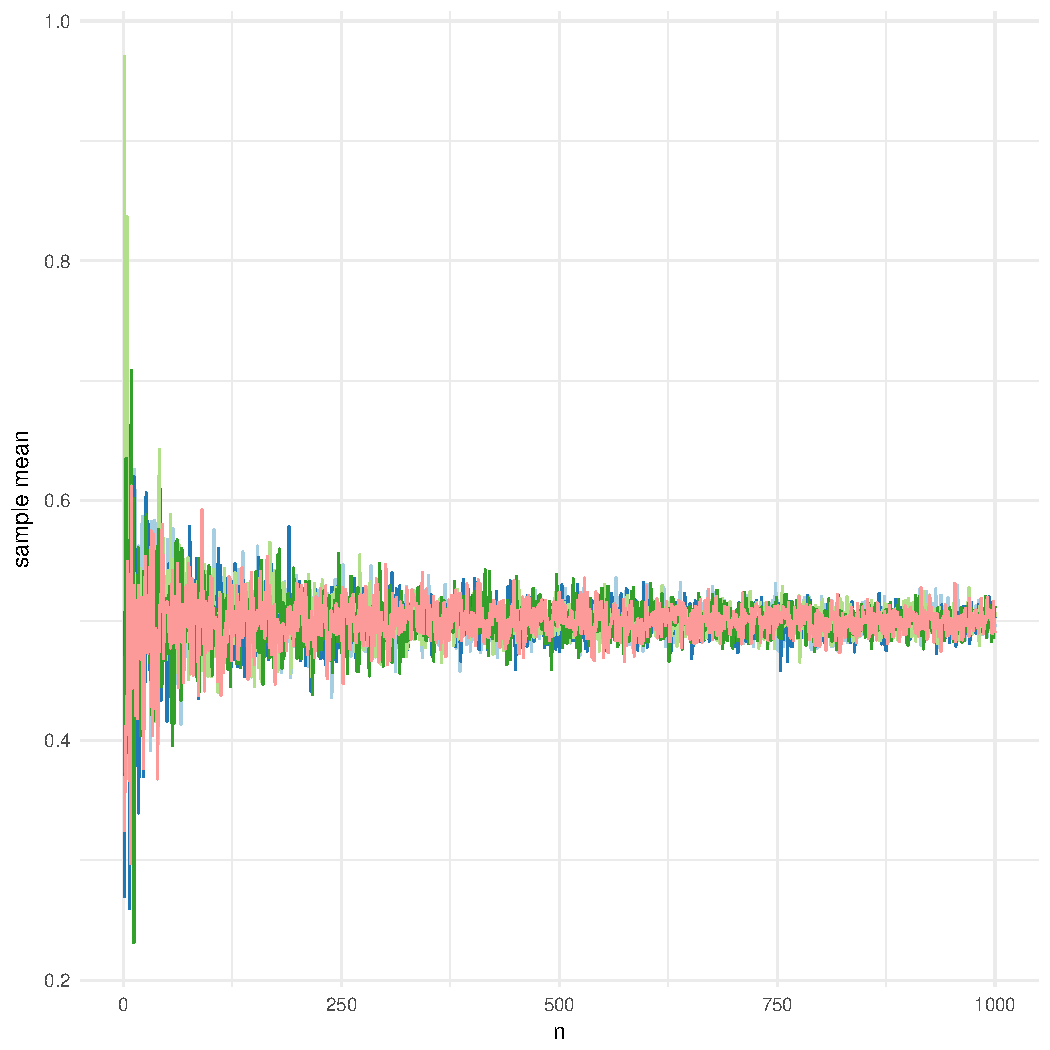
\includegraphics[height=\figheight,width=\figwidth]{llnPlot}
\end{frame}

%%%%%%%%%%%%%%%%%%%%%%%%%%%%%%%%%%%%%%%%%%%%%%%%%%%%%%%%%%%%%%%%%%%%%%

\begin{frame}[allowframebreaks]
  \frametitle{Convergence in probability: examples}
  \begin{itemize}
  \item $\bar{y} \inprob \Er[y]$ by LLN
  \item Sample variance: 
    \begin{align*}
      \hat{\sigma}^2 = & \frac{1}{n} \sum_{i=1}^n (y_i - \bar{y})^2 \\
      = & \underbrace{\frac{1}{n} \sum_{i=1}^n y_i^2}_{\inprob
        \Er[y^2] \text{ by LLN}} -
      \underbrace{\bar{y}^2}_{\inprob  \Er[y]^2 \text{ by LLN and CMT}} \\
      \inprob & \Er[y^2] - \Er[y]^2 = \Var(y)
    \end{align*}
  \item Mean divided by variance:
    \begin{align*}
      \frac{\sum_{i=1}^n y_i}{\sum_{i=1}^n (y_i - \bar{y})^2} = & \frac{\frac{1}{n}
        \sum_{i=1}^n y_i}{\frac{1}{n} \sum_{i=1}^n (y_i - \bar{y})^2}
      \\ 
      = & \frac{\bar{y}}{\hat{\sigma}^2} \\
      \inprob & \frac{\Er[y]}{\Var{y}} \text{ by above and Slutsky's lemma}
    \end{align*}
  \framebreak
  \item Sample correlation:
    \begin{align*}
      \hat{\rho} = & \frac{\frac{1}{n} \sum_{i=1}^n (x_i - \bar{x})(y_i - \bar{y})}
      {\sqrt{\frac{1}{n} \sum_{i=1}^n (x_i - \bar{x})^2 
          \frac{1}{n} \sum_{i=1}^n(y_i - \bar{y})^2}}
    \end{align*}
    \begin{itemize}
    \item 
      $\frac{1}{n} \sum_{i=1}^n (x_i - \bar{x})^2 \inprob \Var(X)$ and 
      $\frac{1}{n} \sum_{i=1}^n(y_i - \bar{y})^2 \inprob \Var(Y)$ as
      above
    \item $\frac{1}{n} \sum_{i=1}^n (x_i - \bar{x})^2 
      \frac{1}{n} \sum_{i=1}^n(y_i - \bar{y})^2 \inprob \Var(X)
      \Var(Y)$ by Slutsky's lemma
    \item $\sqrt{\frac{1}{n} \sum_{i=1}^n (x_i - \bar{x})^2 
        \frac{1}{n} \sum_{i=1}^n(y_i - \bar{y})^2} \inprob
      \sqrt{\Var(X) \Var(Y)}$ by CMT
    \item $\frac{1}{n} \sum_{i=1}^n (x_i - \bar{x})(y_i - \bar{y})
      \inprob \Cov(X,Y)$ by similar reasoning as for sample variance
    \item $\hat{\rho} \inprob \corr(X,Y)$ by Slutsky's lemma
    \end{itemize}
  \end{itemize}
\end{frame}

\subsection{Convergence in distribution}

\begin{frame}[allowframebreaks]\frametitle{Convergence in distribution}
  \begin{itemize}
  \item Convergence in probability tells us that an estimator will eventually
be very close to some number (hopefully the parameter we're trying to
estimate), but it does not tell us about the distribution of an
estimator. 

\item From the law of large numbers, we know that $\bar{y}_n - \mu$
converges to the constant 0. 
\item The central limit theorem tells us that
if we scale up the difference by $\sqrt{n}$, then $\bar{y}_n - \mu$
converges to normal distribution with variance $\Var(y) = \sigma^2$. 
\item Let $F_n$ be the CDF of $W_n$ and $W$ be a random variable
    with CDF $F$
  \item $W_n$ \alert{converges in distribution} to $W$, written $W_n \indist
    W$, if $\lim_{n \to \infty} F_n(x) = F(x)$ for all $x$ where $F$
    is continuous 
  \item \alert{Central limit theorem}: Let $\{y_1, ..., y_n\}$ be i.i.d.
    with mean $\mu$ and variance $\sigma^2$ then $Z_n =
    \sqrt{n} \frac{\bar{y}_n - \mu}{\sigma}$ converges in distribution
    to a standard normal random variable
    \begin{itemize}
    \item As with the LLN, the i.i.d. condition can be relaxed if
      additional moment conditions are added
    \item
      \href{http://en.wikipedia.org/wiki/File:Convergence_in_distribution_(sum_of_uniform_rvs).gif}
      {Demonstration}
    \end{itemize}
  \item Properties:
    \begin{itemize}
    \item If $W_n \indist W$, then $g(W_n) \indist g(W)$ for
      continuous $g$ (\alert{continuous mapping theorem (CMT)})
    \item Slutsky's theorem: If $W_n \indist W$ and $Z_n \inprob c$, then (i) $W_n +
      Z_n \indist W + c$, (ii) $W_n Z_n \indist c W$, and (iii)
      $W_n/Z_n \indist W/c$
    \end{itemize}
 

\item The central limit theorem can be paraphrased as ``scaled and centered
sample means converge in distribution to normal random
variables.'' 

\item ``Scaling'' refers to the fact that we multiple by
$\sqrt{n}$. 

\item ``Centering'' refers to the subtraction of the population
mean. 

\item If an estimator converges in distribution to a normal
random variable, then we often say that the estimator is
asymptotically normal. 
 \end{itemize}
\end{frame}
%%%%%%%%%%%%%%%%%%%%%%%%%%%%%%%%%%%%%%%%%%%%%%

%\begin{frame}[fragile,shrink]
  %\frametitle{Demonstration of CLT}
  %\begin{lstlisting}

%\end{lstlisting} %$
%\end{frame}

%\begin{frame}
  %\frametitle{Demonstration of CLT}

  %\includegraphics[height=\figheight,width=\figwidth]{cltPlot}

%\end{frame}


\begin{frame}[allowframebreaks]
  \frametitle{CLT examples}
  \begin{itemize}
  \item Mean: $\sqrt{n}\frac{\bar{y} - \mu}{\sigma} \indist N(0,1)$ by CLT
  \item What if $\sigma$ estimated instead of known? 
    \begin{align*}
      \sqrt{n} \frac{\bar{y} - \mu}{\hat{\sigma}} 
    \end{align*}
    \begin{itemize}
    \item $\hat{\sigma} \inprob \sigma$ from before
    \item $\sqrt{n}(\bar{y} - \mu) \indist N(0,\sigma^2)$ by CLT
    \item Slutsky's theorem  with $W_n = \sqrt{n}(\bar{y} - \mu)$,
      $Z_n = \hat{\sigma}$ gives
      \[ \sqrt{n} \frac{\bar{y} - \mu}{\hat{\sigma}} \indist N(0,1) \]
    \end{itemize}
  \end{itemize}
\end{frame}

\begin{frame}[allowframebreaks]
  \frametitle{CLT examples}
  \begin{itemize}
  \item Variance: 
    \begin{itemize}
    \item 
      \begin{align*}
        \hat{\sigma}^2 = & \frac{1}{n} \sum_{i=1}^n (y_i - \bar{y})^2 \\
        = & \frac{1}{n} \sum_{i=1}^n (y_i - \mu + \mu - \bar{y})^2 \\
        = & \left[\frac{1}{n} \sum_{i=1}^n (y_i - \mu)^2\right] -
        (\bar{y} - \mu)^2 \\
      \end{align*}
    \item So
      \begin{align*}
        \sqrt{n}( \hat{\sigma}^2  - \sigma^2) = & \sqrt{n}
        \left[\frac{1}{n} \sum_{i=1}^n (y_i - \mu)^2 - \sigma^2 \right]
        - \sqrt{n}(\bar{y} - \mu) (\bar{y} - \mu) 
      \end{align*}
    \item $\sqrt{n}(\bar{y} - \mu) \indist N(0,\sigma^2)$, $(\bar{y} -
      \mu)  \inprob 0$, so $\sqrt{n}(\bar{y} - \mu) (\bar{y} - \mu)
      \indist 0$
    \item CLT implies $\sqrt{n}
      \left[\frac{1}{n} \sum_{i=1}^n (y_i - \mu)^2 - \sigma^2
      \right] \indist N(0,V)$       
    \end{itemize}
  \end{itemize}
\end{frame}

\section{Hypothesis testing}

\begin{frame}[allowframebreaks] 
  \frametitle{Hypothesis testing}
  \begin{itemize}
  \item The main way we will use the central limit theorem is to use the
asymptotic distribution of an estimator to approximate the estimator's
finite sample distribution. 

\item We do this so that we can make
(approximate) statements about how uncertain we are about a given
estimate. 

\item Hypothesis testing is one way we make statements about how random is
an estimate. 
\item The logic hypothesis testing is slightly awkward. 
\item To understand it, keep in mind that we are trying to learn about a
parameter.
\item  Parameters are fixed characteristics of a population. They
are not random. 
\item Therefore, it makes no sense to talk about the
probability that a parameter is a certain value or in a certain
range. 
\item What is random, is the sample that we observe and the estimate
that we calculate from the sample. 
\item Therefore, we can calculate the
probability that our estimate is a certain value in some range. 
\item The probability that an estimate takes on a value depends on the true
population parameter. 
\item Therefore, we generally quantify the randomness
of an estimate by making statements like, assuming the true parameter
is $\theta_0$, then the probability of getting an estimate as far or
farther from $\theta_0$ than the one we observe is $p$. 


  \item \alert{Null hypothesis}, $H_0$
  \item \alert{p-value}: if null hypothesis what is the probability of
    a sample as or more extreme than what is observed
  \item From your previous courses: if $y_i \sim N(\mu,\sigma^2)$, then $\sqrt{n}
    \frac{\bar{y} - \mu}{\hat{\sigma}^2} \sim t(n-1)$ 
  \end{itemize}
\end{frame}

\subsection{Examples}

\begin{frame}[allowframebreaks]
  \frametitle{Example: testing mean}
  \begin{itemize}
  \item From 325: 
    \begin{itemize}
    \item If $y_i \sim N(\mu,\sigma^2)$, then $\sqrt{n}
      \frac{\bar{y} - \mu}{\hat{\sigma}} \sim$ t distribution with
      $n-1$ degrees of freedom
    \item p-value for $H_0: \mu = \mu_0$ vs $H_a: \mu \neq \mu_0$ is 
      \begin{align*} p = & \Pr\left( \abs{\frac{\frac{1}{n} \sum_{i=1}^n y_i -
              \mu_0}{ s_y}} \geq
          \abs{\frac{\bar{y} - \mu_0}{\hat{\sigma}} } \right) \\ 
        = & 2 
        \underbrace{F_t\left(-\abs{\frac{\bar{y} - \mu_0}{\hat{\sigma}}};n-1\right)
        }_{\text{CDF of t distribution}} 
      \end{align*}
    \end{itemize}
  \item What if distribution of $y_i$ unknown?
    \begin{itemize}
    \item Use CLT to approximate distribution of t-statistic
    \end{itemize}
  \end{itemize}
\end{frame}

\begin{frame}
  \frametitle{Example: testing one mean}
  \begin{itemize}
  \item From earlier slide,
    \[ \sqrt{n} \frac{\bar{y} - \mu}{\hat{\sigma}} \indist N(0,1) \]
  \item So,
    \[ \Pr\left( \abs{\frac{\frac{1}{n} \sum_{i=1}^n y_i -
          \mu_0}{ s_y}} \geq
      \abs{\frac{\bar{y} - \mu_0}{\hat{\sigma}} } \right) \to
    2\underbrace{\Phi\left(-\abs{\frac{\bar{y} -
            \mu_0}{\hat{\sigma}}}\right)}_{\text{ standard normal
        CDF}} 
    \]
  \end{itemize}
\end{frame}

\begin{frame}
  \frametitle{Data on deworming treatment and school participation
    from \citet{miguel2003}}

  \begin{tabular}{lcc}
    & Treatment & Control \\
    Sample size\footnote{Only the sample size for observations
      of infections. The real data has more observations of school
      participation, but for illustration we will pretend this is the
      sample size.} & 873 & 352 \\
    Infection & 0.32 & 0.54 \\
    School attendance & 0.808 & 0.684 
  \end{tabular}  

\end{frame}
  
\begin{frame}[shrink]
  \frametitle{Example: testing one mean}
  \begin{itemize}
  \item Test $H_0: \Er[\text{infected}|\text{control}] = 0.5$ againt
    $H_a: \Er[\text{infected}|\text{control}] \neq 0.5$
    \begin{itemize}
    \item Let $I_{i} = 1$ if infected, else $0$
    \item What is sample variance of $I_i$?
      \begin{align*}
        \hat{\sigma}_I^2 = \frac{1}{n} \sum_{i=1}^n (I_i - \bar{I})^2 = & \left(\frac{1}{n}
          \sum_{i=1}^n I_i^2\right) - \bar{I}^2 \\
        = &  \left(\frac{1}{n} \sum_{i=1}^n I_i \right) - \bar{I}^2
        \;\text{ }\; (I_i^2 = I_i) \\
        = & \bar{I} - \bar{I}^2 = \bar{I}(1-\bar{I})
      \end{align*}
    \item Test statistic
      \[ z = \sqrt{n} \frac{\bar{I} - 0.5}{\sqrt{\bar{I}(1-\bar{I})}} =
      \sqrt{352} \frac{0.54 - 0.5}{\sqrt{0.54(1-0.54)}} = 1.506 \]
    \item P-value $ = 2(1-\Phi(z)) = 0.132$
    \end{itemize}
  \end{itemize}
\end{frame}

\begin{frame}
  \frametitle{Example: testing two means}
  \begin{itemize}
  \item Often want to test difference between two means
    \begin{itemize}
    \item $H_0:$ treatment has no effect $\sim$ $H_0$ treatment mean $
      = $ control mean
    \end{itemize}
  \item Let $\mu_T = $ treatment mean, $\mu_C = $ control mean
  \item $H_0: \mu_T = \mu_C$
  \item CLT implies 
    \[ \sqrt{n_T} (\bar{I}_T - \mu_T) \indist N(0,
    \sigma_T^2) \text{ and } \sqrt{n_C} (\bar{I}_C - \mu_C) \indist N(0,
    \sigma_C^2) \]
    i.e.\ $\bar{I}_T $ is approximately $N(\mu_T, \sigma_T^2/n_T)$ 
  \item Sum of two normals is normal
  \item If treatment and control groups independent, then
    $\bar{I}_T - \bar{I}_C $ is approximately $N(0, \sigma_T^2/n_T +
    \sigma_C^2/n_C)$ formally we could show
    \begin{align*}
      \frac{\bar{I}_T - \bar{I}_C}{\sqrt{\hat{\sigma}_T^2/n_T  + \hat{\sigma}_C^2/n_C}} \indist N(0,1)
    \end{align*}
  \end{itemize}
\end{frame}

\begin{frame}
  \frametitle{Example: testing two means}
  \begin{itemize}
  \item Test $H_0: \Er[\text{infected} | \text{control} ] =
    \Er[\text{infected} | \text{treatment}]$ against
    $H_a: \Er[\text{infected} | \text{control} ] >
    \Er[\text{infected} | \text{treatment}]$ 
    \begin{itemize}
    \item Test statistic:
      \begin{align*} 
        z = & \frac{\bar{I}_T - \bar{I}_C}{\sqrt{\hat{\sigma}_T^2/n_T  +
          \hat{\sigma}_C^2/n_C}} \\ = &
      \frac{0.32 - 0.54}{\sqrt{0.32(1-0.32)/873 + 0.54*(1-0.54)/352}} =
      -7.12 
    \end{align*}
  \item P-value $ = \Phi(z) =5 \times 10^{-13}$
    \end{itemize}
  \item Test $H_0: \Er[\text{school} | \text{control} ] =
    \Er[\text{school} | \text{treatment}]$ against
    $H_a: \Er[\text{school} | \text{control} ] <
    \Er[\text{school} | \text{treatment}]$ 
    \begin{itemize}
    \item Test statistic:
      \begin{align*}
        z = & \frac{\bar{S}_T - \bar{S}_C}{\sqrt{\hat{\sigma}_T^2/n_T  +
            \hat{\sigma}_C^2/n_C}} \\ = &
        \frac{0.808 - 0.684}{\sqrt{0.808(1-0.808)/873 +
            0.684*(1-0.684)/352}} = 4.41
      \end{align*}
    \item P-value $ = 1-\Phi(z) =5 \times 10^{-6}$
    \end{itemize}
  \end{itemize}  
\end{frame}

\begin{frame}\frametitle{Example: RAND health insurance experiment}
\begin{itemize}
\item The RAND health insurance experiment randomly assigned 3985 Americans
to one of 14 different insurance plans from 1974-1982. 
\item All insurance
plans included catastrophic coverage --- families total health-care
spending beyond a proportion of their income was completely
covered. 
\item The least generous plan in the experiment only had
catastrophic coverage. 
\item The most generous plan offered comprehensive
care for free. 
\item There were also plans that had a deductible of \$150
per person or \$450 per family, after which everything was
covered. 
\item Finally, there were plans with coinsurance that required
families to pay between 25\% and 50\% of the cost of health care out
of pocket, up to the catastrophic limit.  
\item You can read more about the
RAND health insurance experiment in chapter 1 of \cite{ap2014} or in
\cite{rand2013}.

%\framebreak
  %\includegraphics[width=\textwidth]{rand-spend.png}
\end{itemize}
\end{frame}

%\begin{frame}\frametitle{Example: RAND health insurance experiment}

  %\includegraphics[width=\textwidth]{rand-head.png} \\
  %\includegraphics[width=\textwidth]{rand-health.png} 

%\end{frame}

%\begin{frame}\frametitle{Example: TRUMP health insurance experiment?}
  %\begin{center}
    %\includegraphics[height=2.6in]{ny-insurance}
  %\end{center}

  %\footnotetext{{\slshape{New Yorker}} daily cartoon, January 5th 2017,
    %\url{http://www.newyorker.com/cartoons/daily-cartoon/thursday-january-5th-health-care?intcid=mod-latest}} 
%\end{frame}

\begin{frame}[allowframebreaks]\frametitle{p-value pitfalls}
  \begin{itemize}
  \item Hypothesis tests and p-values are a tool for quantifying
    uncertainty, but not the only tool
  \item Significance thresholds often over-emphasized
  \item Difference in significance is not necessarily a significant
    difference
    \begin{itemize}
    \item $A$ statistically significantly different from $0$ and $B$
      not statistically significantly different from $0$ does not
      imply that $A-B$ is statistically significant
    \end{itemize}
  \item When testing many hypotheses, likely to find significant
    results by chance alone
    \begin{itemize}
    \item Researcher degrees of freedom and garden of forking paths
      can introduce many tests inadvertently
    \end{itemize}
   \item These ideas are frequently discussed by the statistician Andrew Gelman
on his blog. \\
\url{http://andrewgelman.com/2005/06/14/the_difference/} \\
\url{http://andrewgelman.com/2011/09/09/the-difference-between-significant-and-not-significant/}
\\
\url{http://andrewgelman.com/2016/01/04/plausibility-vs-probability-prior-distributions-garden-forking-paths/}
\\
\url{http://andrewgelman.com/2013/11/06/marginally-significant/}
  \end{itemize}
\end{frame}



\subsection{Asymptotic interpretation of p-values}


\begin{frame}\frametitle{Asymptotic interpretation of p-values}
  \begin{itemize}
 \item  When we calculate p-values using the asymptotic distribution of an
estimator, then in a given sample, we know that our p-value is not
exactly correct. 
\item However, we also know that for a sufficiently large
sample, the error in the p-value will be arbitrarily small. 
\item Exactly
how large of a sample we need for the error to be negligible depends
on the true distribution of our sample and the number of parameters we
estimated to calculate the p-value. 
  \item CLT: under $H_0$,
    \begin{align*}
      z_n = \sqrt{n} \frac{\bar{y} - \mu}{\hat{\sigma}} \indist
      N(0,1)  
    \end{align*}
    or equivalently,
    \begin{align*}
      \lim_{n \to \infty} \Pr(z_n \leq x) = \Phi(x)
    \end{align*}
  \item P-values are only correct asymptotically (for large samples)
  \item Small finite sample p-values will be somewhat off
  \item With exact p-values, under $H_0$, p-values from distributed
    $U[0,1]$
  \item Asymptotic p-values, under $H_0$, p-values only $U[0,1]$ in
    large samples
  \end{itemize}
\end{frame}

%\begin{frame}\frametitle{Convergence of $\Pr(z_n \leq x)$} 

  %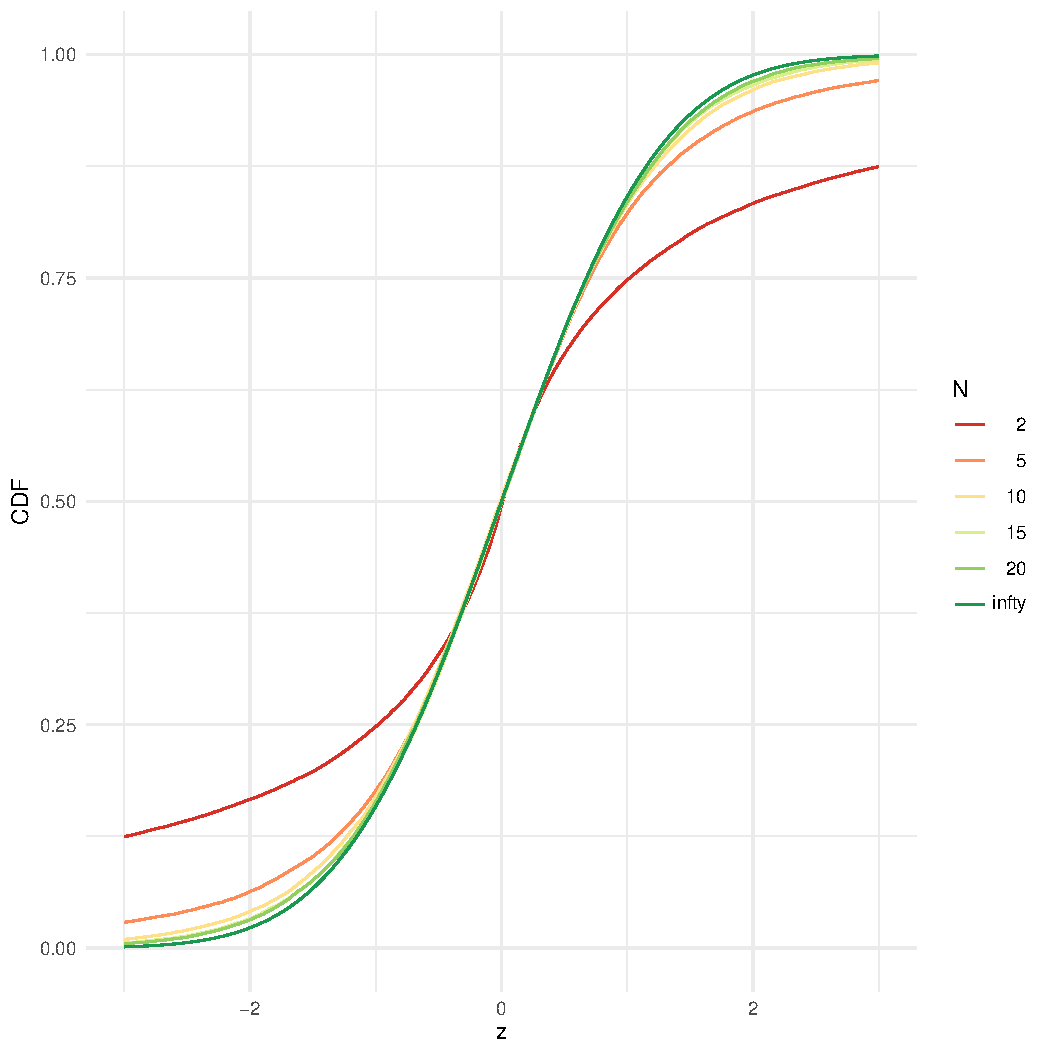
\includegraphics[height=\figheight,width=\figwidth]{clt-cdf}

%\end{frame}

\begin{frame} \frametitle{Convergence of p-values}

  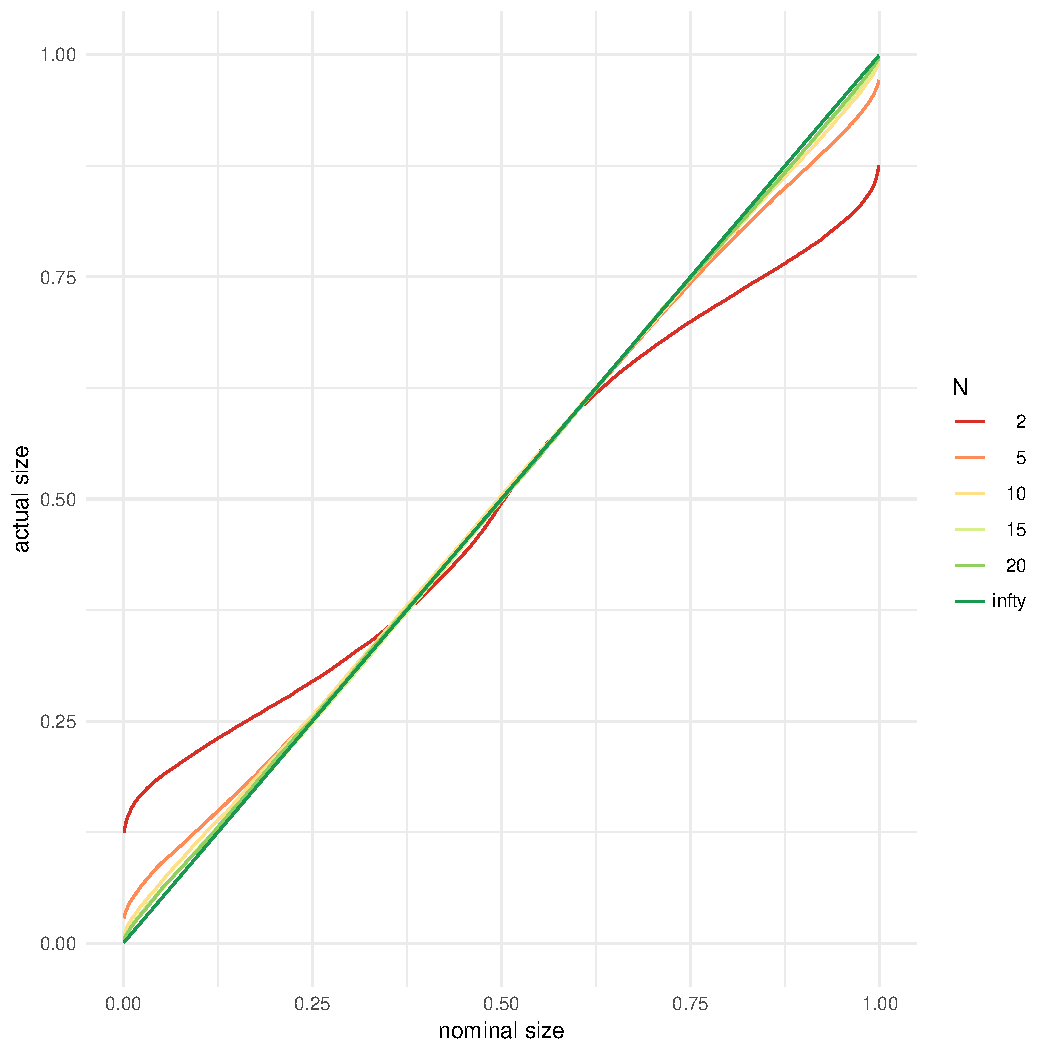
\includegraphics[height=\figheight,width=\figwidth]{clt-p}

\end{frame}

%\begin{frame} 

  %\href{https://bitbucket.org/paulschrimpf/econ326/src/master/notes/02/clt-cdf.R?at=master}
  %{Code for graphs}

%\end{frame}


\begin{frame}[allowframebreaks]
  \frametitle{References}
 \bibliographystyle{jpe}
\bibliography{../UGA_M1_Eco1_biblio}
\end{frame}


\end{document}